\section{Application Categorization}\label{sec:appl}

To first analyze the applications and profile them , we used PIN~\cite{pin} binary instrumentation tool. The PIN tool was modelled to account for total instructions in the application, instructions which get hit in the cache and instructions which actually access memory. 
This profiling was done mainly to account for
which frequency to scale (CPU or DRAM) based on the application information. 
We did not model the Disk (I/O) instructions, as PIN cannot model file system accesses, and
we have no control over the speed at which DISK accesses happen. So, our focus is
mainly on 3 categories:

\begin{itemize} 
\item \textit{Compute Intensive}: The application which spend their time in CPU core and have
more instructions between load/stores to memory. For these applications, CPU
frequency is the important parameter.
\item \textit{Cache Sensitive}: The applications which have more memory access instructions,
but due to the locality of the data accesses, most of them get the data in CPU caches.
For these applications, again CPU frequency is important. It is possible that just
profiling the memory related instructions could be misleading as you do not want to
scale DRAM frequency for cache-senstive applications.
\item \textit{Memory Bound} These are the applications, which have lot of cache misses
and the accesses reach memory. Increasing CPU frequency for these applications could 
lead to wastage of energy. 
\end{itemize}

Figure ~\ref{fig:appl-cat} shows the application categorization across 7 SPEC2006~\cite{spec2006} benchmarks, 5 SPLASH2~\cite{splash2} benchmarks and 2 micro-benchmarks. From the figure it is clear that
SPEC2006 benchmarks are mostly compute intensive, SPLASH2 workloads are Compute and cache sensitive, whereas the 2 micro-benchmarks 
have lot of memory accesses.

Now, we analyzed these workloads with Linux "Ondemand" power governor and 2 power governors of recent Intel P-state driver. 


\begin{figure*}
  \begin{center}
    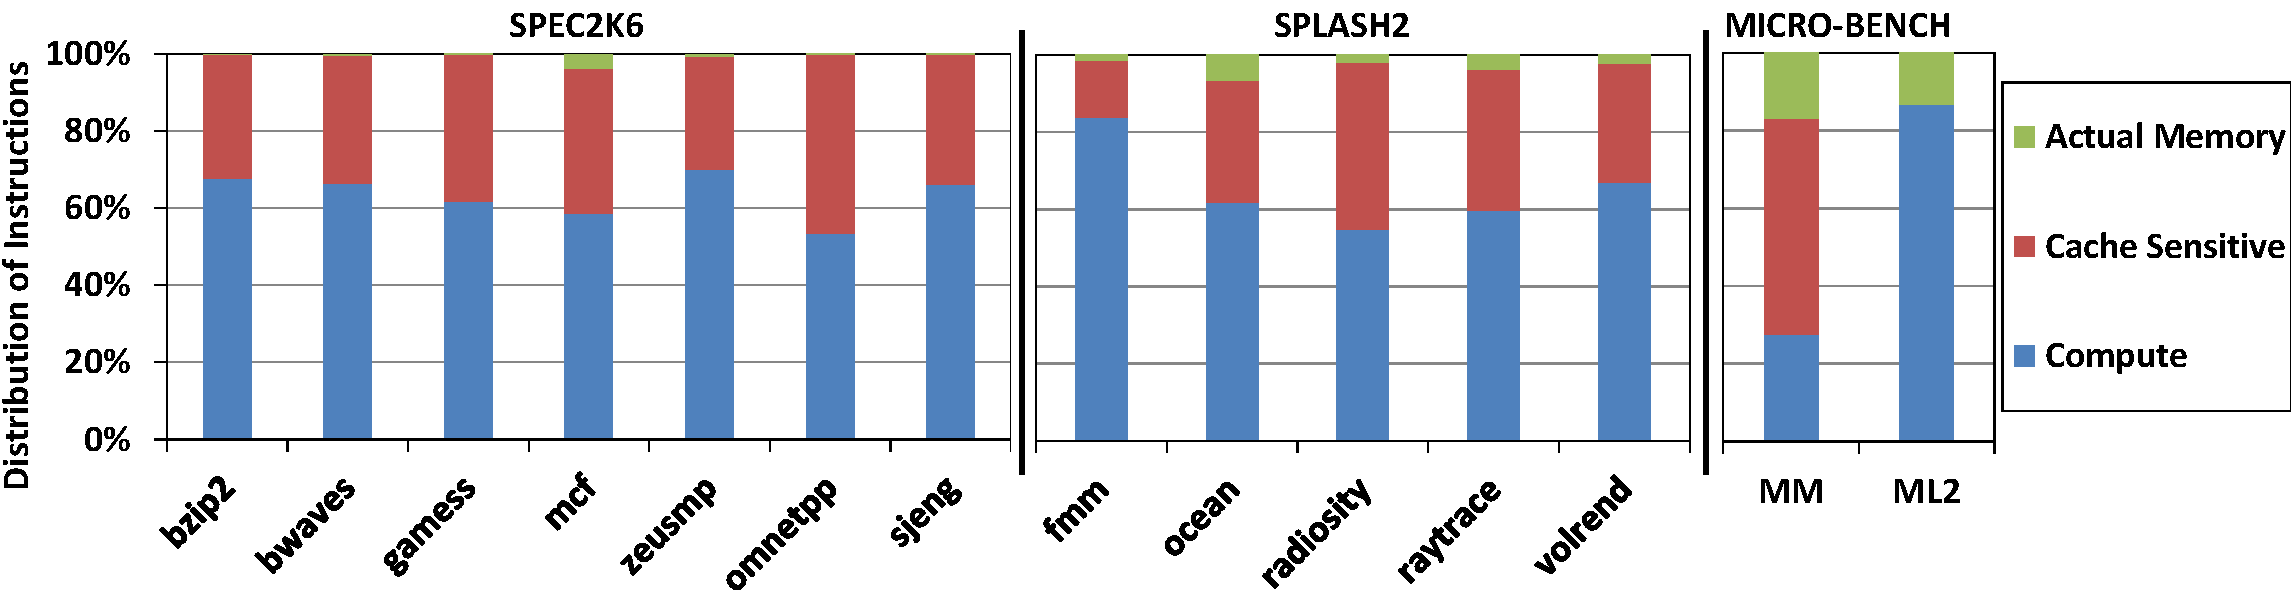
\includegraphics[width=\linewidth]{figs/app-cat-crop.pdf}
  \end{center}
  \vspace{-0.05in}
  \caption{Application Categorization}
  \vspace{-0.04in}
  \label{fig:appl-cat}
\end{figure*}


\begin{figure*}
  \begin{center}
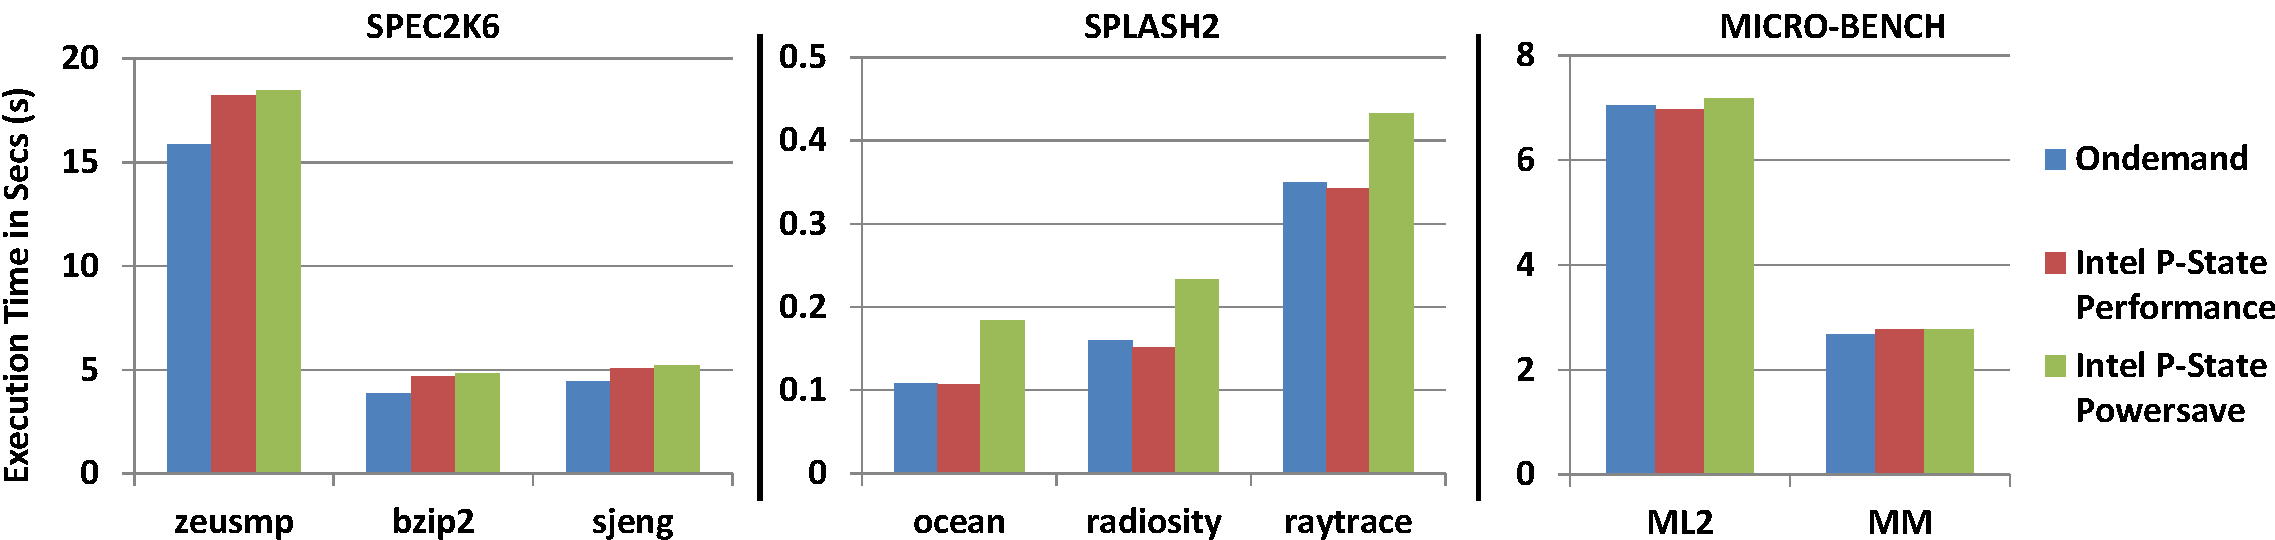
\includegraphics[width=\linewidth]{figs/def-exec-time-crop.pdf}
  \end{center}
  \vspace{-0.1in}
  \caption{Default Linux Drivers Energy}
  \label{fig:sched-results}
\end{figure*}


\begin{figure}
  \begin{center}
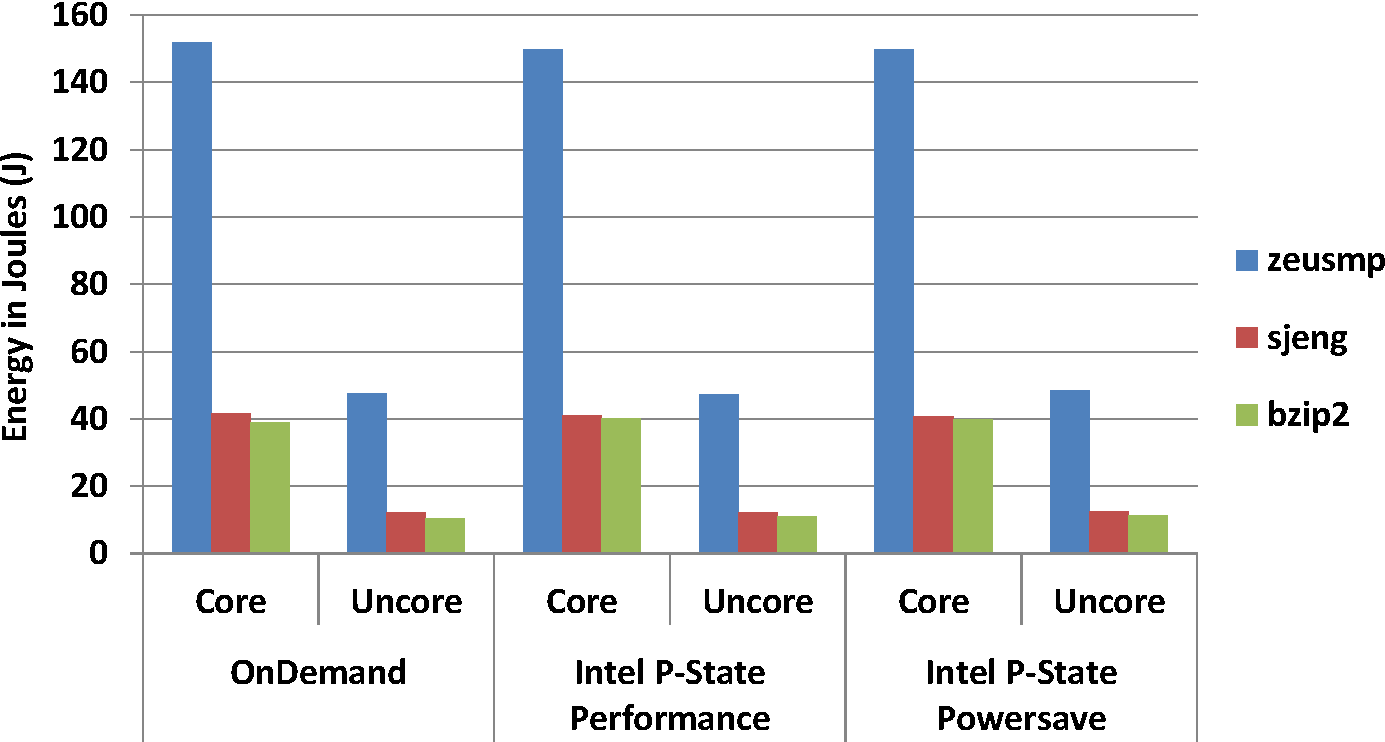
\includegraphics[width=\linewidth]{figs/def-drivers-spec-crop.pdf}
  \end{center}
  \vspace{-0.1in}
  \caption{Default Linux Drivers Energy}
  \label{fig:sched-results}
\end{figure}

\begin{figure}
  \begin{center}
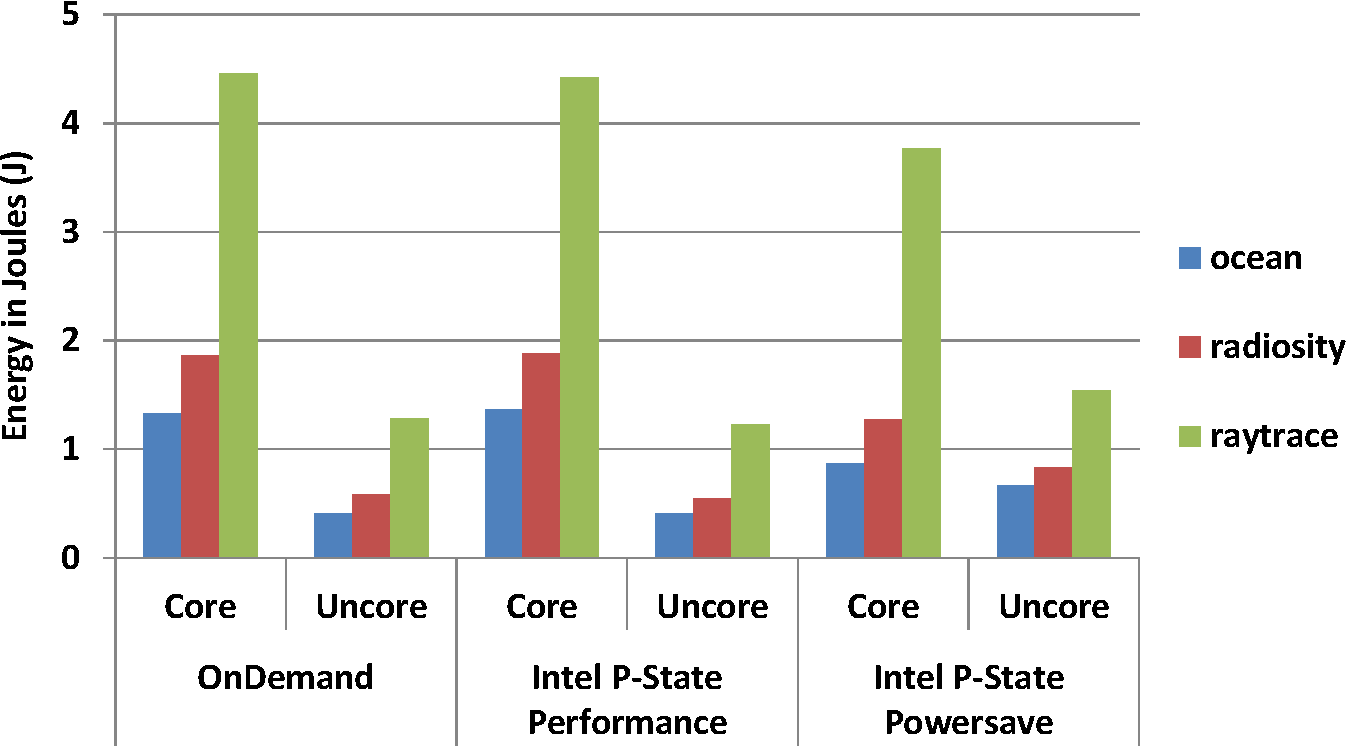
\includegraphics[width=\linewidth]{figs/def-drivers-splash-crop.pdf}
  \end{center}
  \vspace{-0.1in}
  \caption{Default Linux Drivers Energy}
  \label{fig:sched-results}
\end{figure}

\begin{figure}
  \begin{center}
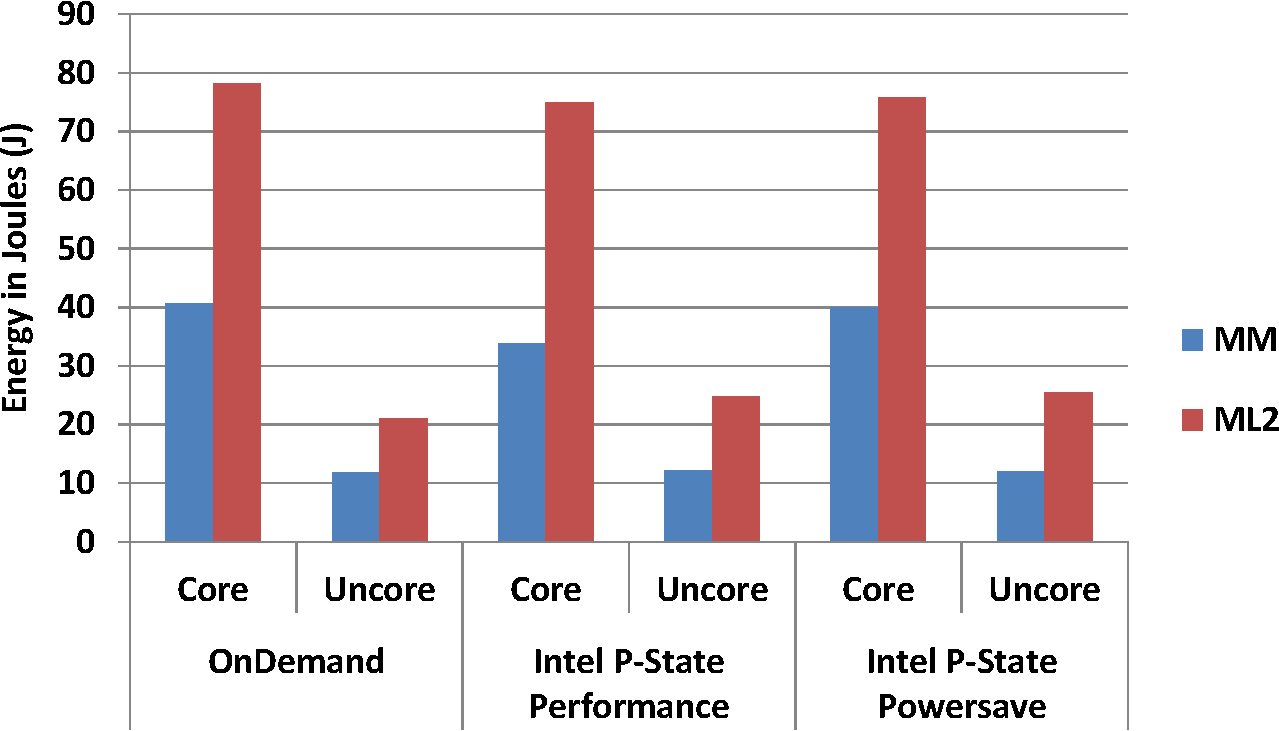
\includegraphics[width=\linewidth]{figs/def-drivers-micro-crop.pdf}
  \end{center}
  \vspace{-0.1in}
  \caption{Default Linux Drivers Energy}
  \label{fig:sched-results}
\end{figure}


